\documentclass[a4paper,11pt]{article}
%@@@@@@@@@@@@@@@@@@@@@@@@@@@@@@@@@@@@@@@@@@@@@@@@@@@@@@@@@@@
%@@@@@@@@@@@@@@@@      PACOTES BÁSICOS		     @@@@@@@@@@
%@@@@@@@@@@@@@@@@@@@@@@@@@@@@@@@@@@@@@@@@@@@@@@@@@@@@@@@@@@@

\usepackage[T1]{fontenc}
\usepackage[utf8]{inputenc}
\usepackage{lmodern} 
\usepackage[portuguese]{babel}
\usepackage{amsmath}
\usepackage{array}
\usepackage{graphicx}				%para imagens
\usepackage{epstopdf} 				%resolve problemas eps-pdf
\usepackage{pict2e}				%%writting to images
%@@@@@@@@@@@@@@@@@@@@@@@@@@@@@@@@@@@@@@@@@@@@@@@@@@@@@@@@@@@
%@@@@@@@@@@@@@@@@     PACOTES NÃO TAOBÁSICOS		 @@@@@@@@@@
%@@@@@@@@@@@@@@@@@@@@@@@@@@@@@@@@@@@@@@@@@@@@@@@@@@@@@@@@@@@
\usepackage{fancyhdr}				% para o cabeçalho bonito
\usepackage{caption}					%para legendas
\usepackage{subcaption}				% e sublegendas
\usepackage{placeins} 				%controlar o lugar dos floats
\pagestyle{fancy} 					% número de pag e cabeçalho
\usepackage{txfonts} 				%fontes bonitas? acho que para o título
\usepackage[usenames]{color} 		% algo com gunplot e eps
\usepackage{ifthen}
\usepackage{xparse}
\graphicspath{{./../images/}{./../data/}{./graph/}}	% procura imagens nessa pasta
\usepackage{float} %%para definir ambiente gráfico
\newfloat{Gráfico}{hbtp}{lop}[section]
%\usepackage{undertilde}	%%para notação de vetor do yuri
\usepackage[import]{xy} % para escrever em imagens
\xyoption{import}

\usepackage{listings}
\lstset{frame=single,}
%@@@@@@@@@@@@@@@@@@@@@@@@@@@@@@@@@@@@@@@@@@@@@@@@@@@@@@@@@@@
%@@@@@@@@@@@@@@@@      Cabeçalho de cada página      @@@@@@@
%@@@@@@@@@@@@@@@@@@@@@@@@@@@@@@@@@@@@@@@@@@@@@@@@@@@@@@@@@@@
\setlength{\headheight}{25pt}%compila sem erro
	\fancyhead{}
	\fancyfoot{}
	\fancyhead[R]{Sistemas de Medição}%direito superior
	\fancyhead[L]{
\includegraphics[height=0.25in]{./../images/logo_unb.pdf}}%esquerda superior
	\fancyfoot[C]{\thepage}%baixo centro
%E: Even page, O: Odd page, L: Left field, C: Center field, R: Right field, H: Header, F: Footer
% em documentos com dois lados use LO, RO. como esse documento não tem lados essa opção é inútil


%@@@@@@@@@@@@@@@@@@@@@@@@@@@@@@@@@@@@@@@@@@@@@@@@@@@@@@@@@@@
%@@@@@@@@@@@@@@@@      NOVOS COMANDOS		      @@@@@@@@@
%@@@@@@@@@@@@@@@@@@@@@@@@@@@@@@@@@@@@@@@@@@@@@@@@@@@@@@@@@@@
\newcommand\undermat[2]
	{
	  \makebox[0pt][l]
	  	{$\smash{\underbrace{\phantom{%
    \begin{matrix}#2\end{matrix}}}_{\text{$#1$}}}$
    		}#2
    	}
    	
\newcommand{\HRule}
	{
	\rule{\linewidth}{0.5mm}
	}
	
\newcommand{\EmptyPage}
	{
	\thispagestyle{empty}
	\mbox{ }
	\newpage	
	} 
	
\newcommand{\MakeMyTitlePage}[4]
%%Argumentos: 
%1º Nome da Matéria
%2º subtítulo ex: experimento IV
%3º título
%4º autores
% exemplo de autores:
%	\begin{center} \large
%		\begin{tabular}{llr} \
%		& & \\[0.05cm]		
%		Professora & Nadia Maria de Liz Koche & \\
%		
%		Alunos:& & \\
%		& Juarez A.S.F 					& 11/0032829\\
%		& Sérgio Fernandes da Silva Reis & 11/0140257\\
%		& Jedhai Pimentel				& 09/0007883\\	[0.05cm]	
%		\end{tabular}
%	\end{center}
{
\begin{titlepage}
\begin{center}

% Upper part of the page. The '~' is needed because \\
% only works if a paragraph has started.

\includegraphics[width=\textwidth]{./../images/logo_unb.pdf}~\\[1cm]

\Huge #1\\[0.5cm]

\huge #2

% Title
\HRule \\[0.4cm]
{ \huge \bfseries  #3}\\[0.4cm]

\HRule \\[0.5cm]

{\large \today}


\vfill %%o que vier depois vai ao fim da páginda


%Autor e Professor
\begin{center} \large
#4
\end{center}

\end{center}
\end{titlepage}

\EmptyPage
\tableofcontents
\newpage

}
	
%@@@@@@@@@@@@@@@@@@@@@@@@@@@@@@@@@@@@@@@@@@@@@@@@@@@@@@@@@@@
%@@@@@@@@@@@@@@@@      NOVOS AMBIENTES		      @@@@@@@@@
%@@@@@@@@@@@@@@@@@@@@@@@@@@@@@@@@@@@@@@@@@@@@@@@@@@@@@@@@@@@
\newcounter{graph-c}
\setcounter{graph-c}{0}


%\NewDocumentEnvironment{Graph}{m}
 % {%antes
  %\addtocounter{graph-c}{1}
  %\begin{figure}
  %}
 %{
 %depois
%	\end{figure} 
%	\caption*{Grafico \arabic{graph-c} - #1}
 %}

















%inclui todosos pacotes utilizados

\newcommand{\MyBox}[1]
{
	\begin{tabular}{|l|}\hline
	  #1 \\ \hline	    
	\end{tabular} 	
}

\begin{document}

%------------------------------------------------------------
%----------------CAPA----------------------------------------
%------------------------------------------------------------

\MakeMyTitlePage
{ProIC 2012/2013}
{Simulação Numérica de Material Granular}
{Relatório Final : Dinâmica Molecular}
{%autores
		\begin{tabular}{llr} \
		& & \\[0.05cm]		
		Orientador: & Yuri Dumaresq Sobral & \\
		
		Aluno:&
		 Juarez A.S.F 					& 11/0032829\\

		\end{tabular}
}

%------------------------------------------------------------
%----------------RESUMO--------------------------------------
%------------------------------------------------------------
\section{Resumo}
\paragraph{}
Estuda-se o desenvolvimento de
um simulador de material granular baseado em dinâmica molecular.
O algoritmo de dinâmica molecular é descrito e detalha-se o
uso de uma tabela de dispersão para a busca eficiente  de
colisões. Os métodos de integração temporal são discutidos e
comparados. Ao final discute-se as principais dificuldades
encontradas na implementação da rotina em C.
%------------------------------------------------------------
%----------------INTRODUÇÃO----------------------------------
%------------------------------------------------------------

\section{Introdução}

  \paragraph{}Materiais granulares são constituídos de uma
  coleção enorme de partículas macroscópicas, por exemplo:
  areia, grãos e o próprio solo. 
  A física que rege o comportamento destes materiais não é
  ainda muito bem entendida. Parte disso se deve ao fato de
  que o movimento global do conjunto  resulta
  do movimento individual de cada partícula e as incontáveis 
  e aleatórias interações que podem ocorrer produzem efeitos
  difíceis de serem analisados. Para ilustrar essa riqueza
  de comportamento, considere o solo que sustenta uma casa. 
  O solo pode ser entendido como a coleção dos grãos e
  rochas que o compõe. Sobre certas condições de umidade e
  compactação ele possui propriedades de um sólido e sustenta
  a casa, sobre outras ele escorre semelhantemente a um
  fluido e a casa desmorona. Nos dois casos as rochas e
  grãos eram os mesmos mas as diferentes condições a que
  estavam submetidos eram diferentes, logo as forças de
  interação entra cada elemento mudaram e o comportamento
  global do composto mudou drasticamente.
  

  \paragraph{}Nesse contexto de um número
  monstruoso de variáveis a serem levadas em consideração, a
  simulação computacional entra como a principal arma para
  atacar o problema. Em muitas situações não temos uma
  fórmula que nos diga o comportamento de um dado material
  granular sob determinadas condições mas uma simulação
  computacional que represente adequadamente as forças
  envolvidas pode nos dar a resposta. Este artigo pretende
  discutir um dos principais métodos utilizados para
  simulação de tais materiais: a dinâmica molecular.

%------------------------------------------------------------
%----------------DINÂMICA MOLECULAR--------------------------
%------------------------------------------------------------
  \section{Dinâmica Molecular}
  \paragraph{} O algoritmo de dinâmica molecular consiste em
  representar o material granular por um modelo discreto de
  partículas elásticas. As forças de contato durante a
  colisão de duas partículas são simuladas permitindo que
  estas  sofram interpenetrações, chamadas de \emph{overlaps},
  e então a lei de Hooke é aplicada para simular as forças
  de restituição e de amortecimento. Colisões são sempre
  resolvidas entre pares e possíveis colisões múltiplas
  são tratadas como colisões entre os pares individualmente e
  independentemente. 
 
  \paragraph{}As principais grandezas físicas utilizadas
  são mostradas na figura \ref{fig:MD}.
  Sejam $\vec{x_1}$ e $\vec{x_2}$ as posições,
  $R_1$ e $R_2$ os raios,  $\vec{v_1}$ e $\vec{v_2}$
  as velocidade  das
  partículas 1 e 2 respectivamente e $\vec{n}$ e
  $\vec{t}$ as direções normais e tangentes. Temos:
  \begin{equation}
    \begin{array}{l}
      \mbox{(overlap)}
              \xi
              = max(0, R_1 + R_2 - |\vec{x_2} - \vec{x_1} |)
\\%	
\mbox{(direção normal)}
          \vec{N} = \frac{\vec{x_2} -
          \vec{x_1} }{|\vec{x_2} - \vec{x_1} |}
\\ %	
\mbox{ (v de aproximação)}\vec{V} = \vec{v_1} - \vec{v_2}
\\%	
\mbox{ (v normal)}  V_n = \dot{\xi} = \vec{V} \cdot \vec{N} 
\\%	
\mbox{ (v tang.)}  \vec{V}_t = \vec{V} - \dot{\xi}\vec{N} 
	\end{array}
    \label{eq:DM-1}
  \end{equation}

  \paragraph{}No algoritmo aqui descrito não nos interessa
  a força na direção tangente causadas por atrito.
  Consideramos portanto as partículas como perfeitamente
  lisas e nos preocupamos
  somente com  a força normal que será dada pela lei de
  Hooke com constante de viscosidade $k_v$ e de restituição
  elástica $k_r$.
    \begin{equation}
		\begin{array}{l}
		    \vec{F}_n = f_n \vec{N}, \\
	    	f_n = -(k_v \xi^\alpha \dot{\xi} + k_r \xi^\beta)
		\end{array}
        \label{eq:DM-2}
    \end{equation}

    \paragraph{}A força descrita pela fórmula acima é a que
    atua na partícula 1 devido a interação com 2. A força
    que atua em 2 tem o mesmo módulo e direção mas sentido
    contrário. No caso mais simples podemos tomar $\beta =
    1$ e $\alpha = 0$. Essas constantes, junto com
    $k_v$ e $k_r$, devem ser
    calibradas para ajustar a fórmula aos dados
    experimentais.

    \paragraph{}A dinâmica molecular nos dá as forças de
    contato devido a colisões. Se conhecermos todas as
    forças externas que atuam sobre a partícula, como peso,
    forças magnéticas e elétricas, estamos
    prontos para aplicar a segunda lei de Newton para cada
    partícula individualmente. 
    
 \begin{equation}
        \sum \vec{F} = \frac{d}{dt} ( m \cdot \vec{v}(t) )
    \end{equation} 
\FloatBarrier

\paragraph{} Para aplicar o algoritmo discretizamos o tempo.
Isto é, não lidamos mais com um tempo contínuo e não nos
preocupamos com a solução analítica, o que procuramos é
acompanhar a evolução do sistema em intervalos de tempo 
$\triangle T$ em $\triangle T$. Nossa simulação, se bem
feita, será tão melhor quanto menor for o passo de tempo
tomado.

\paragraph{}Dadas condições
iniciais para as posições, velocidades e acelerações e
conhecendo-se 
as forças externas atuantes, o algoritmo consiste em para cada
instante de tempo tomado:
\begin{itemize}
  \item atualizar a posição e a velocidade baseado nas
    velocidades e acelerações do instante anterior
  \item procurar e calcular todas as colisões do sistema
  \item somar as forças de colisão com as forças externas
  \item calcular a aceleração a ser usada no próximo passo
    de tempo.
\end{itemize}

\paragraph{} Uma vez dado um par de partículas em colisão o
cálculo das forças é bem simples, bastam as operações
vetoriais descritas em \ref{eq:DM-1} e \ref{eq:DM-2}. O complicado é procurar
por colisões de modo eficiente. Os algoritmos para a
integração das velocidades e posições e para a busca
eficiente de
colisões serão os temas das seções seguintes. 

\begin{figure}[H]
\centering
        \setlength{\unitlength}{0.05\textwidth}
          \begin{picture}(10,9)
                \put(0,0){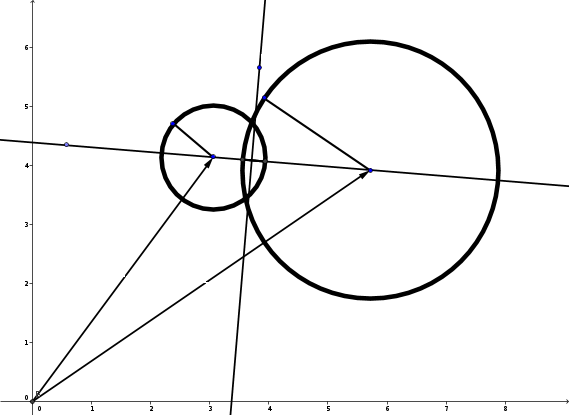
\includegraphics[width=0.5\textwidth]{./images/fig_1-1.png}}
                \put(2.5,3.5){$ \vec{x_1}$}
                \put(3.0, 2.5){$\vec{x_2}$}
                \put(5.2, 5.0){$\vec{R_2}$}
               \put(3.2, 4.8){$\vec{R_1}$}
                \put(4.3, 4.4){$\xi$}

          \end{picture}
	%	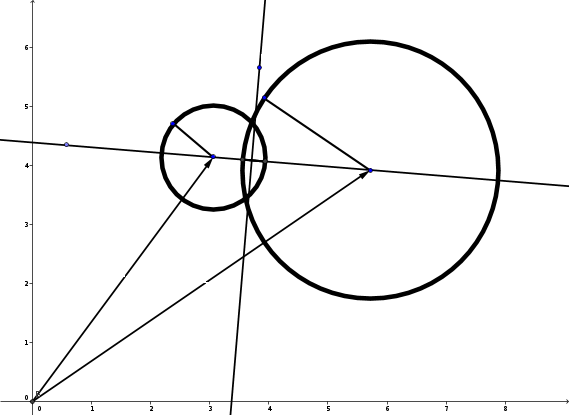
\includegraphics[width = 6 cm]{./images/fig_1-1.png}
		\caption{Principais grandezas utilizadas}
		\label{fig:MD}
\end{figure}
\FloatBarrier

%------------------------------------------------------------
%----------------PROCURANDO POR COLISÕES---------------------
%------------------------------------------------------------

\section{Procurando por colisões}
\paragraph{}A busca por colisões consiste em medir a
distância entre duas partículas e verificar se ela
é menor do que a soma dos raios das duas
partículas. Dadas duas partículas, o único modo de saber se
elas estão ou não em colisão seria medindo a distância entre
elas. O processo é simples mas se torna trabalhoso uma vez
que a princípio todas as partículas do universo são
candidatas a colidirem entre si. É preciso
filtrar os pares de partículas candidatos a colisão. Isso
pode ser feito segmentando o plano em quadrados como na 
figura \ref{fig:hash}. Se cada quadrado tiver lado de comprimento igual
a duas vezes o raio da maior partícula,
temos certeza de que uma partícula só pode colidir com
aquelas que estiverem ou no seu próprio quadrado ou 
nos quadrados adjacentes. Computacionalmente isso pode
ser feito por meio de uma tabela de dispersão. 

\paragraph{}A tabela de dispersão é uma estrutura de dados,
isto é, uma maneira particular de armazenar e
operar dados de modo a utilizá-los eficientemente. Ela
mapeia um dado a uma posição de memória através de uma
função de dispersão. A função de dispersão atua não sobre o
dado em si, mas sobre uma chave atribuída a ele. A principal
vantagem dessa estrutura é que ela permite buscas
extremamente eficientes: conhecendo-se a chave do objeto a
ser procurado, o custo da busca é O(1). Um dos problemas que
surgem na implementação é quando objetos diferentes com
chaves diferentes ou não são mapeados para a mesma posição de
memória. Isso pode ser contornado, por exemplo,
utilizando-se listas para armazenar os elementos que caem na
mesma posição de memória. Lista é uma outra estrutura de
dados cuja principal característica é permitir o
armazenamento sequencial de uma quantidade inicialmente não conhecida
de dados. Em nossa aplicação os dados são as partículas e 
as chaves suas posições no plano. A função de dispersão não
é única e depende muito do sistema que se quer simular, aqui
sugerimos uma para ser usada na simulação de partículas presas
em uma caixa quadrada de comprimento conhecido.

\paragraph{} Seja L o lado da caixa e $R_{max}$ o raio da maior partícula
sendo simulada. Para facilitar vamos tomar o lado da caixa como um múltiplo
inteiro m do maior diâmetro, isto é, $ L = m(2R_{max})$. Vamos colocar as 
extremidades da caixa nos pontos (0,0), (0,L), (L,L), (L,0). Seja $\pi$ o 
pontilhamento:

\begin{displaymath}
  \pi = \{ 0 = x_0, x_1, \ldots, x_k, \ldots, x_{m} = L \}, x_k = k\cdot2R_{max} 
\end{displaymath}

e considere os conjuntos $\sigma_{x_i}$ dados por 

\begin{displaymath}
\sigma_{x_i} = \{x \in R, x_i < x \leq x_{i+1}\}, i = 0,1,\ldots, m-1
\end{displaymath}

\paragraph{}É claro que se uma partícula de centro (x,y) pertence à 
caixa, então sua abscissa x pertence a um e somente um dos conjuntos
$\sigma_{x_i}$ acima. De forma análoga sua ordenada y pertence a somente um dos
conjuntos $\sigma_{y_j}$ que segmentam o eixo y. Dessa forma temos associado ao
ponto (x,y) do plano a dupla (i,j). Veja que a caixa de lado L está dividida em 
m linhas e m colunas e portanto temos $m^2$ pares (i,j) possíveis. Para mapear
cada par em uma posição de um vetor estático de tamanho $m^2$ podemos usar
a função:

\begin{eqnarray}
    p(i,j) = i\cdot m + j
\end{eqnarray} 

\paragraph{}Dessa forma a função acima mapeia todas as partículas que tiverem centro nas posições
$(x_i < x \leq x_{i+1}, y_j < y \leq y_{j+1})$ para a mesma
posição de memória. Cada posição de memória representa um quadrado
no plano, ou seja, o processo descrito implementa
a segmentação do plano discutida anteriormente. 
Quando quisermos buscar os candidatos à colisão devemos olhar somente
as partículas que estão nos quadrados vizinhos, isso é feito jogando
para a função de dispersão os centros dos quadrados vizinhos e buscando 
nas posições retornadas.É claro que nem todas as partículas dos quadrados adjacentes
e mesmo do próprio quadrado estão em colisão, mas reduzimos drasticamente a área do plano
que possui partículas candidatas a colisão. No caso médio o algoritmo é extremamente
mais eficiente do que medir a distância entre todas as partículas.

\paragraph{}Para um dado instante de tempo temos então um algoritmo que permite
achar eficientemente as partículas em colisão. Certa dificuldade surge quando 
incrementamos o tempo e as partículas se movem. Para que a estrutura continue 
funcionando adequadamente precisamos atualizar também a posição da partícula 
na estrutura. Aqui existem duas possibilidades: podemos verificar qual partícula 
saiu dos limites do seu quadrado e então reinseri-la na tabela ou simplesmente 
destruir toda a tabela e construir outra com as novas posições. A primeira opção
economiza custo computacional pois nas simulações uma partícula mantém seu centro
dentro de um mesmo quadrado por muitas interações enquanto a segunda permite
implementação muito mais simples.

\paragraph{}Para tornar a execução ainda mais eficiente, podemos, em vez de ficar
andando com as próprias partículas pela tabela, andarmos com apontadores para partículas. 
Ou seja, os dados da tabela não são todas as informações sobre a partícula e sim
um ponteiro para seu endereço de memória. Dessa forma todo o processo de transferência
de dados de um lugar para o outro se torna mais eficiente.

\paragraph{}Uma outra estratégia que pode ser usada no lugar de olharmos os 9 quadrados
adjacentes é simplesmente inserir as partículas em todos
os 9 quadrados. Dessa forma a busca de colisões precisa olhar somente para os quadrados
individualmente e não para um quadrado e seus adjacentes. Essa escolha no entanto dificulta
o processo de manutenção da tabela entre uma iteração e outra, sendo muito mais adequada
para ser utilizada quando entre um instante e outro destruímos toda a tabela. Para as 
simulações realizadas com cerca de dez mil partículas não houve diferença perceptível entre
esse método e o outro. 

\paragraph{}Para finalizar, é importante que as partículas sendo simuladas mantenham-se
na caixa, nosso ambiente de controle. Uma maneira de fazer isso seria definir as paredes
como retas e definir um algoritmo de colisão entre partículas e retas semelhante
ao descrito na dinâmica molecular. Outra abordagem interessante e muito mais simples é
cobrir as paredes com partículas imóveis. Elas são partículas iguais às outras mas 
simplesmente não calculamos forças sobre elas e não atualizamos suas posições. É importante
notar que não necessariamente as colisões irão impedir que uma partícula passe através da 
outra. Para que isso não aconteça é importante que as constantes estejam bem ajustadas,
principalmente o incremento de tempo. Dessa forma é preciso ter cuidado com as partículas
que venham a furar a caixa: quando isso ocorrer elas devem ser retiradas da simulação, 
ou ao menos da tabela, para que não tenhamos falhas de segmentação.

\paragraph{}Sumarizando, para simular N partículas em uma caixa quadrada de lado L
com $m^2$ divisões iguais temos:
\begin{itemize}
  \item  um vetor estático \textbf{P}
  \footnote{vetor estático:
tamanho conhecido que não se altera ao longo da simulação, permite acesso direto} 
  de tamanho N que guarda os dados sobre as partículas como massa, posição, velocidade
 , aceleração, forças \ldots
  \item uma tabela de dispersão que constitui-se de um vetor estático de tamanho $m^2$
   de listas de ponteiro para partículas. 
   \item A tabela é usada para reduzir o número
   de pares de partículas candidatos a colisão. As colisões são calculadas e os dados
   atualizados no vetor \textbf{P}. São os ponteiros para as partículas que andam na tabela, 
   não as partículas em si.
\end{itemize} 

\paragraph{}Para comparar nosso algoritmo com o algoritmo trivial realizamos uma
simulações com diferentes números de partículas. Deixamos um bloco denso de
partículas cair e colidir com o solo como na figura \ref{fig:simulation}.
Dizemos que o bloco é denso pois as partículas adjacente são tangentes umas 
às outras. Medimos o tempo de simulação começando com 50 partículas e aumentando
de 50 em 50 até uma simulação com 500 partículas para os dois algoritmos. Os 
dados obtidos são mostrados na figura \ref{fig:hash-time-comparsion} junto com
regressões para as curvas. As regressões são:
\begin{displaymath}
  \begin{array}{ll}
  C_{hash}(n) = 0.115758 n + 1.466667
 & \mbox{ (algoritmo Hash)} \\
  C_{trivial}(n) = 0.000774 n^{2} + (-0.004864) n + (1.916666)
 & \mbox{ (algoritmo trivial)} \\
  \end{array}
\end{displaymath}
Vemos que para poucas partículas o algoritmo trivial é mais eficiente mas esse
comportamento é rapidamente invertido. Além disso o algoritmo trivial apresenta
comportamento quadrático como esperado e nosso algoritmo baseado em hashsing
apresenta comportamento linear e de baixo coeficiente angular.


 \begin{figure}[!htp]
	\centering
	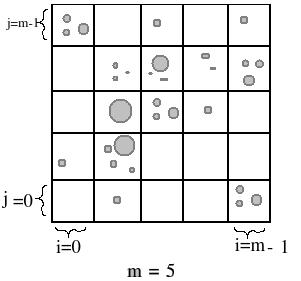
\includegraphics[scale=0.8]{./images/hash.jpeg}
	\caption{Segmentação do plano}
	\label{fig:hash}
\end{figure}
\vspace{-5 cm}
\begin{figure}
	\centering
	% GNUPLOT: LaTeX picture with Postscript
\begingroup
  \fontfamily{phv}%
  \selectfont
\definecolor{t}{rgb}{0.5,0.5,0.5}
  \makeatletter
  \providecommand\color[2][]{%
    \GenericError{(gnuplot) \space\space\space\@spaces}{%
      Package color not loaded in conjunction with
      terminal option `colourtext'%
    }{See the gnuplot documentation for explanation.%
    }{Either use 'blacktext' in gnuplot or load the package
      color.sty in LaTeX.}%
    \renewcommand\color[2][]{}%
  }%
  \providecommand\includegraphics[2][]{%
    \GenericError{(gnuplot) \space\space\space\@spaces}{%
      Package graphicx or graphics not loaded%
    }{See the gnuplot documentation for explanation.%
    }{The gnuplot epslatex terminal needs graphicx.sty or graphics.sty.}%
    \renewcommand\includegraphics[2][]{}%
  }%
  \providecommand\rotatebox[2]{#2}%
  \@ifundefined{ifGPcolor}{%
    \newif\ifGPcolor
    \GPcolortrue
  }{}%
  \@ifundefined{ifGPblacktext}{%
    \newif\ifGPblacktext
    \GPblacktextfalse
  }{}%
  % define a \g@addto@macro without @ in the name:
  \let\gplgaddtomacro\g@addto@macro
  % define empty templates for all commands taking text:
  \gdef\gplbacktext{}%
  \gdef\gplfronttext{}%
  \makeatother
  \ifGPblacktext
    % no textcolor at all
    \def\colorrgb#1{}%
    \def\colorgray#1{}%
  \else
    % gray or color?
    \ifGPcolor
      \def\colorrgb#1{\color[rgb]{#1}}%
      \def\colorgray#1{\color[gray]{#1}}%
      \expandafter\def\csname LTw\endcsname{\color{white}}%
      \expandafter\def\csname LTb\endcsname{\color{black}}%
      \expandafter\def\csname LTa\endcsname{\color{black}}%
      \expandafter\def\csname LT0\endcsname{\color[rgb]{1,0,0}}%
      \expandafter\def\csname LT1\endcsname{\color[rgb]{0,1,0}}%
      \expandafter\def\csname LT2\endcsname{\color[rgb]{0,0,1}}%
      \expandafter\def\csname LT3\endcsname{\color[rgb]{1,0,1}}%
      \expandafter\def\csname LT4\endcsname{\color[rgb]{0,1,1}}%
      \expandafter\def\csname LT5\endcsname{\color[rgb]{1,1,0}}%
      \expandafter\def\csname LT6\endcsname{\color[rgb]{0,0,0}}%
      \expandafter\def\csname LT7\endcsname{\color[rgb]{1,0.3,0}}%
      \expandafter\def\csname LT8\endcsname{\color[rgb]{0.5,0.5,0.5}}%
    \else
      % gray
      \def\colorrgb#1{\color{black}}%
      \def\colorgray#1{\color[gray]{#1}}%
      \expandafter\def\csname LTw\endcsname{\color{white}}%
      \expandafter\def\csname LTb\endcsname{\color{black}}%
      \expandafter\def\csname LTa\endcsname{\color{black}}%
      \expandafter\def\csname LT0\endcsname{\color{black}}%
      \expandafter\def\csname LT1\endcsname{\color{black}}%
      \expandafter\def\csname LT2\endcsname{\color{black}}%
      \expandafter\def\csname LT3\endcsname{\color{black}}%
      \expandafter\def\csname LT4\endcsname{\color{black}}%
      \expandafter\def\csname LT5\endcsname{\color{black}}%
      \expandafter\def\csname LT6\endcsname{\color{black}}%
      \expandafter\def\csname LT7\endcsname{\color{black}}%
      \expandafter\def\csname LT8\endcsname{\color{black}}%
    \fi
  \fi
  \setlength{\unitlength}{0.0500bp}%
  \begin{picture}(5668.00,4534.00)%
    \gplgaddtomacro\gplbacktext{%
      \csname LTb\endcsname%
      \put(774,576){\makebox(0,0)[r]{\strut{} 0}}%
      \put(774,918){\makebox(0,0)[r]{\strut{} 20}}%
      \put(774,1259){\makebox(0,0)[r]{\strut{} 40}}%
      \put(774,1601){\makebox(0,0)[r]{\strut{} 60}}%
      \put(774,1943){\makebox(0,0)[r]{\strut{} 80}}%
      \put(774,2285){\makebox(0,0)[r]{\strut{} 100}}%
      \put(774,2626){\makebox(0,0)[r]{\strut{} 120}}%
      \put(774,2968){\makebox(0,0)[r]{\strut{} 140}}%
      \put(774,3310){\makebox(0,0)[r]{\strut{} 160}}%
      \put(774,3651){\makebox(0,0)[r]{\strut{} 180}}%
      \put(774,3993){\makebox(0,0)[r]{\strut{} 200}}%
      \put(882,396){\makebox(0,0){\strut{} 50}}%
      \put(1378,396){\makebox(0,0){\strut{} 100}}%
      \put(1873,396){\makebox(0,0){\strut{} 150}}%
      \put(2369,396){\makebox(0,0){\strut{} 200}}%
      \put(2865,396){\makebox(0,0){\strut{} 250}}%
      \put(3360,396){\makebox(0,0){\strut{} 300}}%
      \put(3856,396){\makebox(0,0){\strut{} 350}}%
      \put(4352,396){\makebox(0,0){\strut{} 400}}%
      \put(4847,396){\makebox(0,0){\strut{} 450}}%
      \put(5343,396){\makebox(0,0){\strut{} 500}}%
      \put(144,2284){\rotatebox{-270}{\makebox(0,0){\strut{}Tempo de execução(s)}}}%
      \put(3112,126){\makebox(0,0){\strut{}Número de partículas}}%
      \put(3112,4263){\makebox(0,0){\strut{}Comparando algoritmos de busca por colisões}}%
    }%
    \gplgaddtomacro\gplfronttext{%
      \csname LTb\endcsname%
      \put(4014,3840){\makebox(0,0)[r]{\strut{}algoritmo baseado em hashing}}%
      \csname LTb\endcsname%
      \put(4014,3660){\makebox(0,0)[r]{\strut{}algoritmo trivial}}%
    }%
    \gplbacktext
    \put(0,0){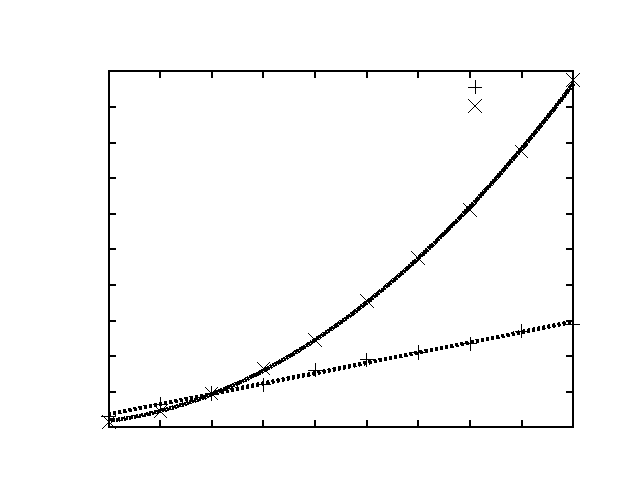
\includegraphics{./../graph/SAC}}%
    \gplfronttext
  \end{picture}%
\endgroup

	\caption{Comparação entre algoritmos de busca}
	\label{fig:hash-time-comparsion}
\end{figure}
\FloatBarrier


\section{Integração Temporal}

\paragraph{} Conhecendo a aceleração e a velocidade de uma partícula em um
instante de tempo podemos calcular a velocidade e a posição no instante
seguinte. Esse processo é dito integração temporal pois corresponde a 
resolver as duas integrais:
\begin{displaymath}
	\begin{array}{l}
		s(t_0+\triangle t) = s(t_0) + \int_{t_0}^{t_0+\triangle t} v(t) dt \\
		v(t_0+\triangle t) = v(t_0) + \int_{t_0}^{t_0+\triangle t} a(t) dt
	\end{array}
\end{displaymath}

A abordagem mais direta corresponde a aproximar o integrando como constante no
intervalo considerado e aproximar:
\begin{displaymath}
	\begin{array}{l}
		s(t_0+\triangle t) \approx s(t_0) + v(t_0)\triangle t  \\
		v(t_0+\triangle t) \approx v(t_0) + a(t_0)\triangle t
	\end{array}
\end{displaymath}

Isso corresponde a utilizar uma aproximação de diferenças finitas de
segunda ordem para a primeira derivada e pode ser mostrado que esse método
de integração é O($\triangle t$). Isto é, espera-se que a aproximação 
melhore linearmente à medida que diminuímos o incremento de tempo. Uma outra
aproximação usando diferenças finitas de ordem mais alta nos leva a um método
de integração mais eficiente de ordem ($\triangle t ^2$):

\begin{displaymath}
	\begin{array}{l}
		s(t_0+\triangle t) \approx s(t_0-\triangle t) + 2v(t_0)\triangle t  \\
		v(t_0+\triangle t) \approx v(t_0-\triangle t) + 2a(t_0)\triangle t
	\end{array}
\end{displaymath}

Veja que esse método requer que guardemos também  informações sobre o instante
de tempo anterior. O ganho na convergência, no entanto, supera esse pequeno
preço.
Métodos de diferenças finitas de ordens mais altas podem se empregados para obter
métodos de integração mais eficientes mas sempre com custo adicional de
utilizar cada vez mais instantes de tempo anteriores. 
 
%------------------------------------------------------------
%----------------IMPLEMENTAÇÃO EM C--------------------------------------
%------------------------------------------------------------
\section{Implementação em C}

\paragraph{}Os conceitos vistos até agora foram implementados na linguagem
C utilizando-se apenas as bibliotecas padrões. Em determinados instantes
de tempo, as posições e demais informações da simulação são impressos
utilizando-se a linguagem para imagens postscript. Esses frames podem então ser 
convertidos em vídeo e a simulação observada.
Na figura \ref{fig:simulation} vemos alguns instantes de uma simulação.Um bloco
com 500 partículas é deixadas cair e atinge o solo com uma certa velocidade.
As paredes da caixa são constituídas cada uma de 4000 mil pequenas partículas 
de forma que na imagem vemos um traço contínuo. Para manter controle da qualidade 
da simulação medimos em todos os instantes de tempo a energia mecânica total 
e o máximo overlap do sistema.

\paragraph{} Como vê-se na figura, nossa simulação com incremento de tempo de
$10^{-5}s$ conseguiu manter uma boa taxa de conservação de energia, mas o overlap
máximo simulado chegou perto de 30\%. Várias simulações foram realizadas
variando-se as constantes do sistema e overlaps máximos pequenos somente
foram obtidos com incrementos de tempo da ordem de $10^{-6}s$. A energia, 
no entanto, foi conservada com incrementos de tempo da ordem de $10^{-4}s$. 

\paragraph{}A principal dificuldade encontrada foi na correta implementação da
tabela de dispersão. Partindo-se somente das bibliotecas padrões em C, toda 
a implementação da tabela e das listas é baseada em ponteiros. Além da
dificuldade em se acertar o complicado uso de ponteiros, a simulação de 
sistemas com muitas partículas trouxe à tona problemas de alocação e desalocação
de memória. Foi preciso manter um controle rígido da alocação para ter-se
certeza de que toda a memória alocada estava sendo liberada, pois pequenas
pontas soltas acabavam por comer toda a memória disponível levando a uma 
falha no programa.No entanto, é preciso dizer que os benefícios da utilização
correta da estrutura de dados eficiente são mais do que evidentes como
mostrado no gráfico \ref{fig:hash-time-comparsion}. 
O trabalho é um exemplo de como uma estrutura de dados, se bem 
implementada, pode ser utilizada para tornar algoritmos muito mais eficientes.

\FloatBarrier
\begin{figure}[!hto]
\hspace{-1 cm}
	\begin{subfigure}{0.5\textwidth}
		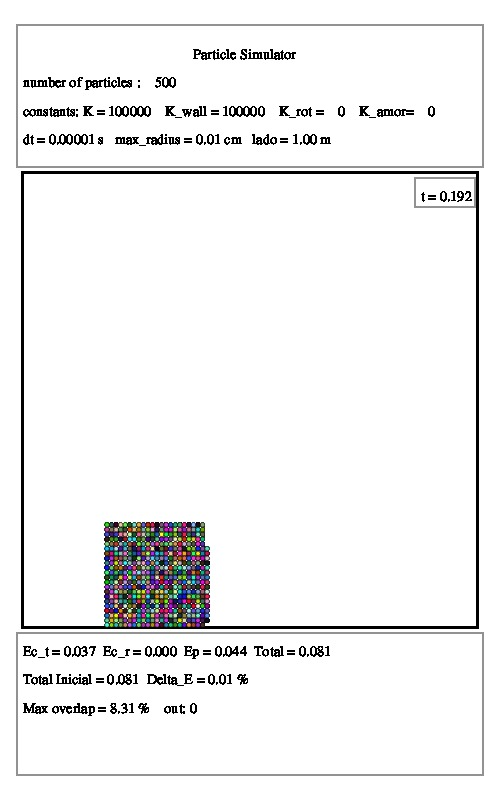
\includegraphics[scale=0.4]{./images/time_0.jpeg}
		\caption{}
	\end{subfigure}
\hspace{2 cm}
	\begin{subfigure}{0.5\textwidth}
		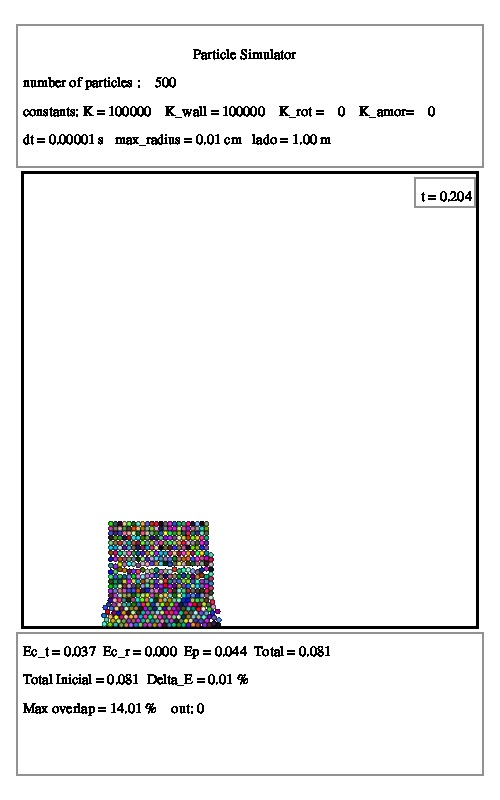
\includegraphics[scale=0.4]{./images/time_1.jpeg}
		\caption{}
	\end{subfigure}
	
\hspace{-1 cm}
	\begin{subfigure}{0.5\textwidth}
		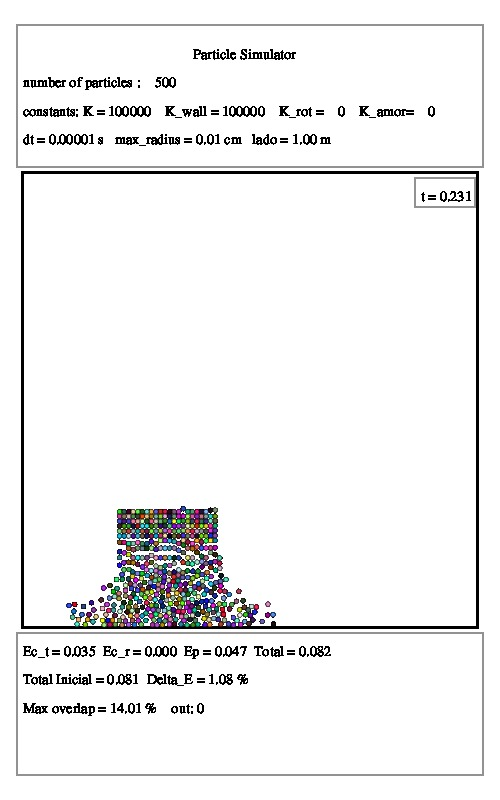
\includegraphics[scale=0.4]{./images/time_2.jpeg}
		\caption{}
	\end{subfigure}
\hspace{2 cm}
	\begin{subfigure}{0.5\textwidth}
		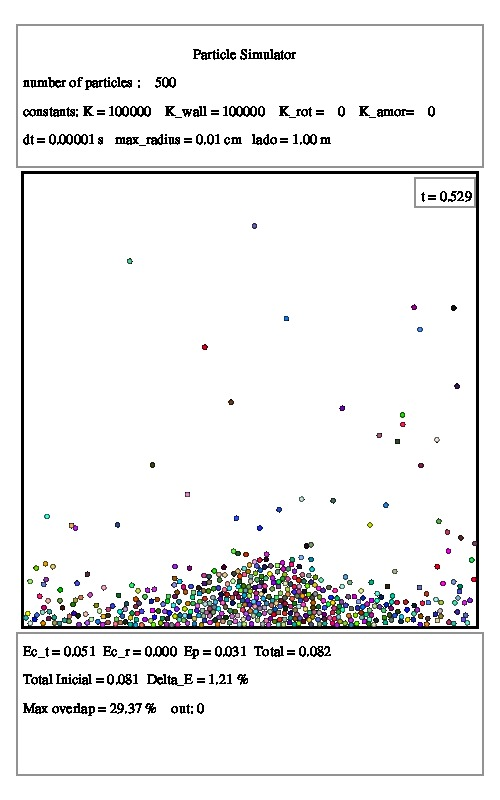
\includegraphics[scale=0.4]{./images/time_3.jpeg}
		\caption{}
	\end{subfigure}
	\caption{Bloco de partículas atinge o solo com constante de amortecimento nula}
	\label{fig:simulation}
\end{figure}
\FloatBarrier




\end{document}
